\chapter{Project Evaluation}\label{sec:project-evaluation}
In this chapter we will first discuss the testing of the system, including automatic testing, acceptance testing evaluating the classifier and evaluating the end results. Afterwards we will evaluate the fulfilment of the requirements. Next we evaluate the fulfilment of the design goals. Then we give the product evaluation and we finnish with the process evaluation.

\section{Validation and Verification}
In this section, we first describe how the system is tested and how we verify the quality of the code with SIG \cite{sig}. Afterwards we define a protocol with which the results of the system can be evaluated for correctness. We will first evaluate the results of the classification, and then the relation scores. These are related in the sense that a relation score is calculated by the number of occurrences in labelled documents, so the correctness of labelling affects the correctness of relation scores.\\

\subsection{Testing the Application}
We will test the program using four different testing methods. As framework we will use pytest\cite{pytest} which is integrated in python. The first is unit testing, which tests the separate components individually. Next comes integration testing, to see how well different components work together. Afterwards we use system testing for testing the different system components. Lastly, acceptance testing is used for testing how well the clients think the program works.

\subsubsection{Unit Testing}
Unit testing is done by writing automatic tests and making sure they pass every time the tests are executed. Unit tests test each method of a function separately, checking that the method does what it is supposed to do. If the method would need information from outside the class that information is mocked. This means that instead of using that other class, a fake object is made which returns a fake value. This ensures the tests will never fail due to changes in other classes. We achieved a test coverage of 85\%.

\subsubsection{Integration Testing}
Integration testing uses automated tests which test how well different components of the system work together. This is done more or less the same as unit testing, however whilst you would mock methods from other classes in unit testing, with integration testing you do not. It is assumed that the separate modules are unit tested, therefor if an error occurs it is because something is wrong with the interaction between the modules and not with the modules themselves. 

\subsubsection{System Testing}
We also used system testing. System testing provides a more complete test of the entire system. This means it is useful to detect faults in the overall system, but less easy to determine where these faults may be located. System testing is done manually, which means the tests can not be easily repeated when the system changes whilst with other testing techniques this is possible.

\subsubsection{Acceptance Testing}\label{sec:acceptance-testing}
Last we used acceptance testing. This is testing done to see if the software does what the clients are expecting it to do. These tests are therefore also executed by the clients manually. Afterwards they can say what worked, what did not work, what was missing and what could be improved. This can for example be used to test if the visualisation looks good to the client.\\

\subsection{SIG}
SIG \cite{sig}, short for software improvement development group, is an organisation that analyses the code of projects to give insights in the quality of how the code is written. A high score means the code is highly maintainable and is kept simple. SIG includes Better Code Hub \cite{bch_guidelines} which checks our code according to 10 guidelines as can be seen in appendix \ref{A_better_code_hub_guidelines}. The great thing about Better Code Hub is that it can be run at anytime. We can check Better Code Hub whenever, whilst for SIG we have to send in our code and wait for feedback. 

\subsubsection{week 5}
The first feedback from SIG was in the fifth week of development. Before uploading on BetterCodeHub our code passed all checks. For SIG it had a score from four out of five stars which means our code is above average maintainable. The last star was missed because the code is above average complex. This means that some of the functionality of some methods should be split into separate methods.

\subsubsection{week 9}
Since the upload date for SIG is the same date as the due date of the final report we can not present the second SIG review. Instead we will present the results from BetterCodeHub, run on the last day before the due date of the report. This time there were two issues which resulted in a score of 8/10. The first was with keeping unit interfaces small, which resulted from a method with too many parameters. However since the different parameters are not part of a same object we did not take time better spent elsewhere to refactor this. The other issue was with coupling architecture components loosely, which resulted from our workers being used for different parts of the application.

\subsection{Evaluating the Classification}
There are several ways to evaluate machine learning algorithms. We will base our evaluation of the classifier on the guidelines of the Microsoft Azure Machine Learning evaluation model \cite{EvualteML}. According to the page binary classification can be evaluated with the following metrics: Accuracy, Precision, Recall, F1 and AUC. Note that we will use a one vs the rest strategy, meaning all classes will be separately evaluated.

\subsubsection{Accuracy}\label{sec:mean-accuracy}
Accuracy is the proportion of correctly classified instances. This however a poor indication of how well the classifier works. For instance if you have a test set of 100 websites, of which 90\% belongs to Category A. Than if the classifier simply predicts all websites to belong to category A the accuracy would be 90\%. It would seem the classifier performs well, but it actually fails to classify the other 10\% of the websites correctly. On average, our classifier had an accuracy of 80 \%.

\subsubsection{Confusion Matrix}
A page can only either belong to class A (positive), or not belong to class A (negative). If a page is predicted by the classifier correctly it is called true positive (TP) or true negative (TN). If the classifier predicts the page incorrectly it results in a false positive (FP) or false negative (FN). This can be seen in the confusion matrix in figure \ref{fig:confusion_matrix}. 

\begin{figure}[ht]
\centering
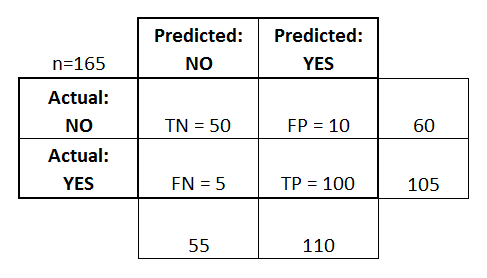
\includegraphics[width=0.5\textwidth]{confusion_matrix}
\caption{confusion matrix \protect\footnotemark{}}
\label{fig:confusion_matrix}
\end{figure}
\footnotetext{\url{https://docs.microsoft.com/en-us/azure/machine-learning/machine-learning-evaluate-model-performance}}


\subsubsection{Precision, Recall, F1 and UAC}\label{sec:classification-validation}
The \textbf{precision} of the classifier is the proportion of positives that are classified correctly: $\frac{TP}{TP+FP}$. This is used for questions such as "Out of the pages that were classified as category A, how many were classified correctly?".\\

the \textbf{recall} of the classifier is used to answer the question "What percentage of the pages that fit category A were classified correctly?". In other words: $\frac{TP}{TP+FN}$.

The \textbf{F1 Score} uses both precision and consideration. It is computed by using the following formula: $F1 = 2\cdot \frac{precision \cdot recall}{precision + recall}$. The F1 score summarised evaluation in a single number, but for evaluation it is better to use recall and precision to understand the behaviour of the classifier. \\

\begin{figure}[ht]
\centering
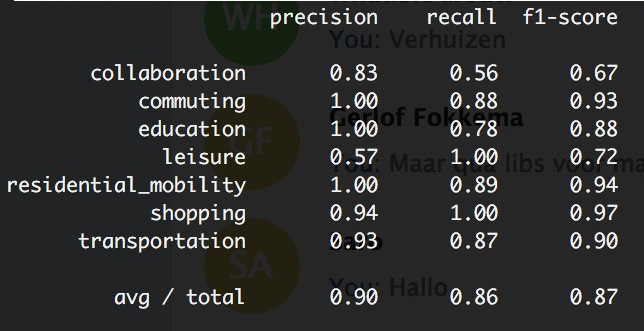
\includegraphics[width=0.5\textwidth]{precision-recall}
\caption{Precision Recall and F1 table}
\label{fig:prec-rec}
\end{figure}

The \textbf{Receiver Operating Characteristic (ROC) curve} and the corresponding \textbf{Area Under the Curve (AUC) value} can be used to inspect the true positive rate (Recall) vs. the false positive rate $\frac{FP}{FP + TN}$. To do this, the possibilities pages are correctly classified are needed. For each threshold on these probabilities for the classifier, the true positive rate and the false positive rate are calculated and are plotted in a graph, which results in something like \ref{fig:UAC}. The closer the ROC curve is to the upper left corner, the better the classifier's performance is. When close to the diagonal of the plot, the classifier tends to make predictions close to random guessing. The UAC value is the are under the ROC curve.

\todo{calculate ROC values and accuracy values?}

\begin{figure}[ht]
\centering
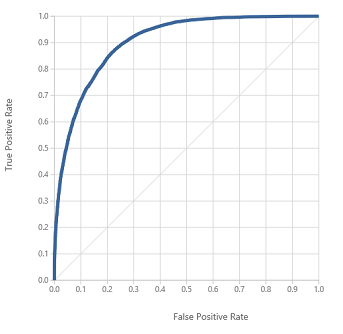
\includegraphics[width=0.5\textwidth]{UAC}
\caption{ROC / UAC graph \protect\footnotemark{}}
\label{fig:UAC}
\end{figure}
\footnotetext{\url{https://docs.microsoft.com/en-us/azure/machine-learning/machine-learning-evaluate-model-performance}}

\subsection{Evaluation of Relation Scores} \label{sec:validation_protocol}
Evaluating relation scores is done differently. An important factor here is that cities have a natural relation due to their geographical position \cite{tobler1970computer}, so one would expect cities that lie close to each other are more related than cities that are on different sides of the country. This natural relation can be represented using the Gravity Model by Reilly \cite{reilly1931law}. The Gravity Model describes that the expected relation between two cities is based on the population of the two cities and the distance between these cities. A relation between two cities that is extracted from the data should thus expose a similar relative score as they would for the gravity model. Consider for example Amsterdam and Hoofddorp, which are cities that lie close to each other. Amsterdam is a large city, whereas Hoofddorp is much smaller. However, due to their close geographical position, the score that results from the Gravity Model would be high. If they turn out to have a very high score in our system, that would imply that the system is correct. Besides the Gravity Model, one can rely on the opinion of an expert in the field of urbanism that can judge whether an extracted relation is close to reality or not. We therefore agreed with the client that they would decide on a small set of relations whether they are correct. Lastly, the relations in the Randstad, a large urban area with the four largest cities of the Netherlands, have been examined before on the basis of firms \cite{van2010economic}. These relations can be compared to those extracted by the system.

\section{Evaluation of Requirements}
In section \ref{sec:reqs} we declared the requirements for our program. Table \ref{requirements_pass/fail} shows which of these requirements passed or failed and why. Failed requirements are discussed in section \ref{sec:Discussion - Open Issues}. As can be seen most of the requirements passed, but there are also some that failed. Most of the failed requirements are acceptable, but the failed must have is planned to be fixed in the last week of coding. Since this is after the due date for this report this fix can not be included in the report.\\

\begin{table}[H]
\centering
\caption{Requirements fulfilment}
\label{requirements_pass/fail}
\begin{tabular}{ll m{8cm}}
\textbf{Must Haves}                     & Pass / Fail & Comment                                                                                                                                                                                                                           \\
1 Mining from Common Crawl     & Pass        & Data is successfully gathered from Common Crawl.                                                                                                                                                                                       \\ \hline
2 Exporting relations          & Fail        & Due to many delays in other parts, exporting the data was not achievable within the time set for the product.                                                                                                                         \\ \hline
3 Extracting relations         & Pass        & Relations are successfully extracted from documents for about 80-85 \%.                                                                                                                                                            \\ \hline
4 Visualisation                & Pass        & A front-end which shows the data on a map is ready for use.                                                                                                                                                                           \\ \hline
5 Present statistics           & Pass        & The front-end presents statistics with the shown data.                                                                                                                                                                                \\ 
                               &             &                                                                                                                                                                                                                                       \\
\textbf{Should Haves}                   & Pass / Fail & Comment                                                                                                                                                                                                                               \\
1 Hierarchical relations       & Fail        & Since extracting relations from text documents was more challenging than first thought, hierarchical relations were not included.                                                         \\ \hline
2 Machine learning retrainable & Pass        & It is possible to retrain the machine learning by feeding it a set of labelled documents.                                                                                                                                              \\ \hline
3 Add large data sets           & Pass        & It is possible to add large  data sets, however since it does cause an increase in time needed to run the algorithm, we did not use a large data set for our demo version.                     \\ \hline
4 Duplicate city names         & Fail        & The algorithm does not take cities with duplicate names, or names fitting to multiple cities into account, due to time constraints.                                                         \\
                               &             &                                                                                                                                                                                                                                       \\
\textbf{Could haves}                    & Pass / Fail & Comment                                                                                                                                                                                                                               \\
1 Use Delpher                  & Fail        & It is not possible to use data from Delpher unless it is already downloaded and stored.                                                                                                                                               \\ \hline
2 Visualisation for comparing  & Pass        & The front-end includes visualisation for comparing cities and relationships to each other.                                                                                                                                            \\
                               &             &                                                                                                                                                                                                                                       \\
\textbf{Would likes}                    & Pass / Fail & Comment                                                                                                                                                                                                                               \\
1 Show all connections         & Fail        & Theoretically it is possible to do this, but it would result in a map on which relationships can not be differentiated from each other due to the large amount the system was not build for (see section \ref{sec:map-clutter}). \\ \hline
2 Other than .nl data          & Fail        & The classifier is only trained on Dutch domains.                                                                 
\end{tabular}
\end{table}

\section{Evaluation of Design Goals}
In section \ref{sec:design-goals} we discussed the design goals for this project. We came up with seven design goals on which we will reflect.

\subsection{Credible}
As can be seen for the classification in section \ref{sec:classification-validation} the classification seems to be pretty good except for the recall value from collaboration and the precision value from leisure. This is most likely due to the low amount of samples. Also when looking at the average the results seem credible.
\todo{add something about ROC values?}

\subsection{Understandable}
From the acceptance tests \ref{sec:acceptance-testing} we resulted that the visualisation as presented in \ref{sec:5-front-end} we devised that the visualisation looks good and is easy understandable.

\subsection{Scalable}
For scalability the goal was to allow the project to be scalable so that websites from other domains than .nl can be used. Since we used Neo4J for storing relationships and Neo4J is highly scalable, storing the relationships for other domains than .nl should not be a problem. 

\subsection{Plugable}
The design goal plugable the goal was to make the application able to perform analysis on different data sets without the need of a developer. Whilst this is possible, the documents from other data sets would have to be in the correct format before they can be processed. For small data sets this might not be that much of a problem, but for larger data sets it would become very time-consuming without the help of a developer.

\subsection{Exportable}
At this moment we have not met the design goal exportable, which was to ensure the numeric data could be exported, for example in CSV format. Since this is not a vital part of the application, this has not yet been included. We are however still working on this. 

\subsection{Fast Development}
Another goal was to have a fast development cycle because of the time constraints. To do this we choose tools, applications and programming languages with which members of our team were already experienced with. Even so, some setbacks occurred which caused the cycle to slow down.

\section{Product Evaluation}
To conclude the two previous sections; we have a functioning program that consists of most vital components. Whilst the results from the application are not exportable (yet), the other design goals were met. The program provides credible and understandable which can be used to analyse relationships between cities in the Netherlands. It can also be extended for non-Dutch cities and pages. Most of the requirements also passed, but depending on the needs of the end-user, it would not be difficult to extend to program to include the others as well. Even though functionality might be missing this is a useful application for analysing data and as a demo it proves systems like these are worth wile to develop.

\section{Process Evaluation}
In this section, we evaluate the development process and explain what methods were used and if they were used correctly. Additionally, we discuss the collaboration with the client and coach and within the group.

\subsection{Development Process Evaluation}
In order to have a smooth development cycle, we made several agreements in the beginning of the project. All code changes had to be submitted through a pull request and needed to be reviewed before they could be merged into the main code base. This was enforced using the project settings in GitHub, where branch access can be regulated. We believe that this approach has helped us greatly to write good quality code and to make sure everyone knew what was going on.

Furthermore, we used Travis CI\footnote{\url{https://travis-ci.org/}} for continuous integration. Building was automatically triggered by both pull requests and normal pushes. GitHub also provides an option to require status checks to pass before being able to merge. However, we disabled this due to some testing stability issues in the first few weeks of development. We did however agree to only merge when all status checks passed. In all but a few hasty merges we managed to adhere to this agreement. Because of the continuous integration of Travis CI, we hardly ever had to deal with unforeseen integration problems of new features.

Travis was also configured to submit coverage reports to Coveralls\footnote{\url{https://coveralls.io}}, so we could easily monitor how test coverage was affected by code changes. Rule of thumb was that all newly added files should have at least 80\% code coverage. Through Coveralls, we could quickly verify this. \todo{add final test code \#lines, coverage \%, etc.}

The product development was managed using the agile development methodology Scrum. Each week was a single sprint. We kept track of the current sprint and the product backlog in Trello\footnote{\url{https://trello.com}}, which helped us to have a clear overview of the product's status. We did however notice that weekly sprints were a bit too short. Usually, a sprint was too full and in the end we noticed that we got somewhat careless about sprints. Moreover, at times, unexpected time consuming issues lead to not finishing the sprint at all. It might therefore be beneficial to extend sprint duration to two weeks to allow for unexpected problems.

The system was initially run on a relatively small virtual private server (4GB RAM, 2 CPUs, 150GB SSD) of one of the group members. With increasing database size, we noticed that we would require more resources, especially RAM. We therefore asked the client to request a server of the TU Delft that we could use for the application. After a few weeks of inefficient (mis)communication, we eventually got access to a 8GB RAM, 4CPUs, 100GB HDD virtual machine. This server meets the minimal requirements for the system, but does not provide enough resources if the data set is extended to more than a million documents. Moreover, the virtualisation is not ideal for the many disk IO the application requires. Therefore, it would have been better to have a physical device at hand.

\subsection{Communication Evaluation}
Communication with the client went very well throughout the entire project. We could always walk into the office with questions or remarks, or email the client if he was not present. He also complimented us whenever he liked something we achieved, but remained critical in his feedback.

The coach and the group had some teething problems but managed to improve quite satisfactory on this. We received useful feedback on both the reports and design. Moreover, she kept forcing us to keep feasibility of our solutions in mind, to make sure we kept aligned with the time schedule.

The group communicated well over the course of the project. We agreed to be present every day of the week between 09:00 and 17:00 to make sure everyone was involved.